\documentclass[11pt]{article} %Tamaño de la letra

%Paquetes esenciales
\usepackage[spanish]{babel}
\usepackage[utf8]{inputenc}
\usepackage[T1]{fontenc}
\usepackage{float}
%Fuente arial
\usepackage{helvet}
\renewcommand{\familydefault}{\sfdefault}

%Hipervinculos y citas
\usepackage{csquotes} %
\usepackage[backend=biber, style=apa, sortlocale=es]{biblatex} % <-- CORREGIDO
\usepackage{hyperref} % <-- CORREGIDO: estaba mal escrito como 'hyperrref'
\usepackage{url}
%Graficos y color
\usepackage{graphicx} % Required for inserting images
\usepackage{xcolor}
\usepackage{tikz}
\usetikzlibrary{arrows.meta}
\usetikzlibrary{positioning}    
\usetikzlibrary{babel}
\usepackage{amsmath}
\usepackage{colortbl}
%Simbologia Matematica
\usepackage{amsmath}
\usepackage{amsfonts} % ← Necesario para \mathbb
\usepackage{amssymb}


%Margenes y espacio
\usepackage[a4paper, left = 2cm, right = 1cm, top=2cm,bottom=2cm]{geometry}
\usepackage{setspace}
\linespread{1.0} %Espacio
\usepackage{setspace}


%Esto cambia el color del fondo
\pagecolor{white} %Cambia este color de las paginas
\color{black} %Cambia el color del texto


%Bibilografia
\addbibresource{referencias.bib}
\begin{document}


% PORTADA
\begin{titlepage}
    \thispagestyle{empty}
    \begin{spacing}{1.5}
    \begin{center}
        
\includegraphics[width=0.2\textwidth]{Images/LogoUNA.svg.png} \\[30pt]
        {\Large \textbf{Universidad Nacional de Costa Rica}} \\[20pt] 
        {\Large Escuela de Informática} \\[20pt]
        {\Large \textbf{Redes Neuronales de Grafos (GNNs)}} \\[20pt]
        {\Large Curso: Estructuras Discretas} \\[20pt]
        
        {\Large \textbf{Estudiantes a cargo de la investigación:}} \\[10pt]
        {\large Sebastián Garro Granados \\ Joel Brenes Vargas \\ Efraín Ignacio Retana Segura} \\[20pt]
        
        {\Large \textbf{Profesor a cargo del curso:}} \\[10pt]
        {\large Carlos Loría-Sáenz} \\[20pt]
        
        {\Large \textbf{NRC:} 41358} \\[5pt]
        {\Large \textbf{Grupo:} 02 – 10:00 a.m.} \\[100pt]
        
        {\Large \textbf{Fecha:} 16 de mayo de 2025}
    \end{center}
    \end{spacing}
\end{titlepage}
    

% RESUMEN
\newpage
{\large \textbf{Resumen}}  
\vspace{5pt}

Este trabajo presenta una investigación introductoria sobre las redes neuronales de grafos (GNNs, por sus siglas en inglés), una combinación de teoría de grafos y aprendizaje automático que ha ganado gran relevancia en la última década. En particular, se investigó una arquitectura específica: las Graph Convolutional Networks (GCNs), las cuales permiten extender los mecanismos de redes neuronales convolucionales (CNNs) al dominio no estructurado de los grafos. Este enfoque resulta útil en aplicaciones donde los datos tienen relaciones o estructuras subyacentes representables mediante nodos y aristas.

El objetivo principal de esta investigación es ofrecer una entrada para que se pueda comprender los fundamentos de las GNNs y vincularlos con los contenidos vistos en clase, especialmente los relacionados con grafos y su programación en Python. Para lograrlo, el trabajo incluye una revisión teórica sobre el aprendizaje supervisado con redes neuronales, conceptos fundamentales de grafos, y una justificación del uso de GNNs frente a modelos tradicionales.

Como parte del desarrollo, se presentan ejemplos demostrativos en Python donde se implementa un ejemplo basico de GCN para resolver una tarea de clasificación de nodos. Estos ejemplos utilizan bibliotecas especializadas y están diseñados para reforzar los aspectos técnicos tratados en el documento. Además, se hace uso de herramientas como GitHub para la gestión del demo, extras y el propio documento de la investigación, Overleaf para la documentación , y entornos de desarrollo compatibles con bibliotecas de aprendizaje profundo.

El informe final busca no solo cumplir con los requerimientos de la investigación, sino también ofrecer una pequeña muestra del gran potencial que representan las GNNs en el campo de la inteligencia artificial moderna.

\vspace{5pt}
\textbf{Palabras clave:} grafos, redes neuronales, GNN, GCN, aprendizaje automático, aprendizaje supervisado,Python,nodos, clasificación de nodos.

\newpage
\tableofcontents
\listoftables
\listoffigures
\newpage
\section{Introducción}
\vspace{5pt}

\subsection{Motivación y Justificación}
\vspace{1pt}
Las Redes Neuronales de Grafos (GNNs) son modelos de aprendizaje profundo hechos para datos con estructura de grafo, donde la relación entre elementos es igual de importante como sus características individuales. Las Redes Convolucionales sobre Grafos (GCNs) aplican operaciones de agregación local en vecindarios de nodos, permitiendo la integración eficiente de información estructural y de atributos, lo que mejora significativamente el desempeño en tareas complejas como clasificación, detección de comunidades y sistemas de recomendación.

Este trabajo analiza el funcionamiento de las GNNs, con especial énfasis en las GCNs, y explora sus aplicaciones en contextos donde la estructura relacional y las dependencias entre datos son fundamentales, como es el caso de las redes sociales y otros sistemas dinámicos.

\vspace{5pt}
\subsection{Objetivo general}
\vspace{1pt}
Analizar el funcionamiento y aplicaciones de las GNNs, enfocándose en el modelo GCN, abordando tanto sus fundamentos teóricos como su uso práctico en escenarios reales de datos estructurados.

\vspace{5pt}
\subsection{Objetivos específicos}
\vspace{-3pt}
\begin{itemize}\setlength\itemsep{0pt}
    \item Describir los conceptos teóricos fundamentales sobre redes neuronales y grafos.
    \item Explicar el mecanismo de propagación y agregación de información en las GCNs.
    \item Implementar una GCN aplicada a un conjunto de datos estructurado en forma de grafo.
    \item Comparar el rendimiento de las GCNs frente a métodos tradicionales de clasificación.
    \item Explorar aplicaciones prácticas de las GCNs en redes sociales y sistemas de recomendación.
\end{itemize}

\vspace{5pt}
\subsection{Alcances del estudio}
\vspace{-3pt}
\begin{itemize}\setlength\itemsep{0pt}
    \item Presentar un marco teórico claro y detallado de las GNNs y GCNs.
    \item Describir el proceso de propagación de información en grafos y la importancia de la estructura de la red.
    \item Implementar una GCN funcional utilizando librerías como PyTorch Geometric o NetworkX.
    \item Evaluar la aplicabilidad y ventajas del modelo en entornos con datos parciales o relaciones complejas.
\end{itemize}

\vspace{5pt}
\subsection{Extras}
\vspace{-3pt}
Se desarrollaron dos extras, cuyos códigos están disponibles en repositorios de GitHub, accesibles para el profesor (usuario: \texttt{CarlosLoriaSaenz}):

\begin{itemize}\setlength\itemsep{1pt}
    \item \textbf{Clasificador MNIST Superpixels:}  
    Clasificador basado en GNN entrenado con el dataset MNIST Superpixels, que convierte imágenes en grafos para su análisis estructurado. Código en:  
    \url{https://github.com/Pachaconjettt/Discretas_pt2}

    \item \textbf{GCN con Dataset Cora:}  
    Implementación de una GCN con PyTorch Geometric para la clasificación de artículos científicos, considerando las relaciones de citación entre ellos. Código en:  
    \url{https://github.com/7joelb/Extra-GCN-DIscretas}
\end{itemize}


% Si no llevas extras, simplemente reemplaza el contenido de la subsección por:
% "No se incluyeron extras en esta investigación."

\newpage
\section{Conceptos de Grafos y sus Aplicaciones}

\subsection{Definiciones}
\begin{itemize}
 \item \textbf{Vértice (Nodo)}: Entidad de un mundo de estudio dado.
 \item \textbf{Arco (Arista)}: Asociación o relación entre vértices.
 \item \textbf{Grafos simples}: No hay dobles arcos entre dos vértices ni lazos.
 \item \textbf{Multigrafo}: Grafo que sí permite dobles arcos, pero no lazos.
 \item \textbf{Seudografos}: Multigrafo con lazos.
 \item \textbf{Grafos dirigidos}: Grafos donde los arcos tienen una dirección.
\end{itemize}
\noindent (Definiciones tomadas de~\cite{carlosloria})

\subsection{Representaciones}

\begin{figure}[H]
\centering
\begin{tikzpicture}[
    nodo/.style={circle, draw=blue, fill=blue!70, minimum size=8mm, inner sep=0pt},
    edge/.style={draw=red, thick},
    every node/.style={font=\small\bfseries, text=blue}
]

% Nodos (posición aproximada)
\node[nodo, label=left:1] (1) at (0,1) {};
\node[nodo, label=left:2] (2) at (0,0) {};
\node[nodo, label=above:3] (3) at (1,1.5) {};
\node[nodo, label=right:4] (4) at (1,0.5) {};
\node[nodo, label=below:5] (5) at (2,0) {};
\node[nodo, label=below:6] (6) at (3,0) {};
\node[nodo, label=above:7] (7) at (3,1) {};
\node[nodo, label=above:8] (8) at (2,1) {};

% Aristas
\draw[edge] (1) -- (2);
\draw[edge] (1) -- (3);
\draw[edge] (2) -- (4);
\draw[edge] (3) -- (4);
\draw[edge] (4) -- (5);
\draw[edge] (4) -- (8);
\draw[edge] (5) -- (6);
\draw[edge] (6) -- (7);
\draw[edge] (7) -- (8);

\end{tikzpicture}
\caption{Representación gráfica de un grafo no dirigido. Fuente: Elaboración propia}
\end{figure}
\begin{figure}[H]
\centering
\begin{tikzpicture}[scale=1, every node/.style={scale=1.3}]
\tikzstyle{nodo}=[
    circle,
    draw=blue,
    fill=blue,
    inner sep=0pt,
    minimum size=8mm % Tamaño de nodo
]
\tikzstyle{rededge}=[-, thick, red]
\tikzstyle{greenedge}=[-, thick, olive]

% Nodos
\node[nodo, label=left:1] (1) at (0,2) {};
\node[nodo, label=left:2] (2) at (0,0) {};
\node[nodo, label=above:3] (3) at (3,3) {};
\node[nodo, label=right:4] (4) at (3,1) {};

% Aristas verdes
\draw[greenedge, bend left=15] (1) to (3);
\draw[greenedge, bend left=15] (1) to (2);
\draw[greenedge, bend left=15] (2) to (4);
\draw[greenedge, bend left=15] (3) to (4);

% Aristas rojas

\draw[rededge, bend left=15] (2) to (1);
\draw[rededge, bend left=15] (4) to (2);


\end{tikzpicture}
\caption{Representación gráfica de un multigrafo. Fuente: Elaboración propia}
\end{figure}

\begin{figure}[H]
\centering
\begin{tikzpicture}[->, >=Stealth, node distance=2cm, thick]
    \tikzstyle{every node}=[circle, draw, fill=blue!20, minimum size=1cm]

    \node (A) {A};
    \node (B) [right of=A] {B};
    \node (C) [below of=A] {C};
    \node (D) [right of=C] {D};
    \node (E) [below of=D] {E};

    \draw (A) -- (B);
    \draw (A) -- (C);
    \draw (B) -- (D);
    \draw (C) -- (D);
    \draw (D) -- (E);
\end{tikzpicture}
\caption{Representación gráfica de un grafo dirigido. Fuente: Elaboración propia}
\end{figure}

\subsection{Métricas Comunes}
Estas son algunas de las métricas de los grafos que se suelen usar en el campo de \textit{Machine Learning} y \textit{Neural Networks}:
\begin{itemize}
    \item \textbf{Grado (Degree)}: Número de conexiones que tiene un nodo.
    \item \textbf{Camino (Path)}: Secuencia de nodos conectados mediante aristas.
    \item \textbf{Centralidad (Centrality)}: Mide la importancia de un nodo dentro de la red.
    \begin{itemize}
        \item \textbf{Centralidad de grado (Degree Centrality)}: Basada en el número de conexiones directas del nodo.
        \item \textbf{Centralidad de intermediación (Betweenness Centrality)}: Basada en la cantidad de caminos más cortos que pasan por un nodo.
        \item \textbf{Centralidad de cercanía (Closeness Centrality)}: Inversa de la suma de las distancias desde el nodo a todos los demás nodos.
    \end{itemize}
    \item \textbf{Coeficiente de agrupamiento (Clustering Coefficient)}: Mide qué tan interconectados están los vecinos de un nodo. 
\end{itemize}
\noindent (Definiciones tomadas de~\cite{mayo2025network})

\subsection{Aplicaciones}
\begin{itemize}
   
\item \textbf{Redes Sociales}:
    El uso de grafos en redes sociales es esencial, ya que nos permite transformar interacciones humanas en datos estructurados en grafos, lo cual permite analizarlas usando teoría de grafos, lo cual ayuda a mejorar experiencias de usuario, prevenir riesgos y entender fenómenos sociales complejos. 
    Según \cite{oracle2024graph}: "Las bases de datos orientadas a grafos se pueden usar en muchos escenarios diferentes, pero normalmente se utilizan para analizar redes sociales. De hecho, las redes sociales son el caso de uso ideal, ya que en ellas intervienen un gran volumen de nodos (cuentas de usuario) y conexiones multidimensionales (interacciones en muchas direcciones diferentes)." Lo cual demuestra el gran poder que nos da el uso de grafos en redes sociales, ya que al estar tantas personas conectadas acelera el análisis de datos y permite un nivel de eficiencia extremadamente alto.
\item \textbf{Grafos de Conocimiento}:
Los grafos de conocimiento son un tipo de grafos que organizan datos interconectados para representar conocimiento de manera semántica, contextual y comprensible no solo para humanos, también para sistemas inteligentes. En vez de almacenar información de forma aislada, conectan entidades (como personas, lugares, conceptos) mediante relaciones que reflejan su significado y contexto. Esto permite mejorar la comprensión automática del lenguaje, realizar inferencias lógicas y ofrecer respuestas más precisas en aplicaciones como buscadores, asistentes virtuales o sistemas de recomendación. 

Según \cite{ibm_knowledge_graph} “un grafo de conocimiento organiza datos interconectados que, juntos, proporcionan una comprensión más rica del significado detrás de la información”, basándonos en esto, se puede ver que los grafos de conocimiento facilitan la toma de decisiones basadas en datos estructurados e interpretables. Gracias a esta capacidad de conectar información dispersa y estructurarla de forma inteligente, los grafos de conocimiento son una herramienta clave para el desarrollo de inteligencia artificial y la transformación digital en múltiples sectores. 
\end{itemize}

\newpage
{\section{Conceptos Básicos de ML usando Redes Neuronales (NNs)}} \vspace{10pt}

\subsection{a.Nociones de Machine Learning (ML)}
\vspace{5pt}

\subsubsection{i. Definición} 
\vspace{3pt}

El \textit{Machine Learning} (ML) es una rama de la inteligencia artificial (IA) que se enfoca en el desarrollo de algoritmos capaces de aprender a partir de datos. En el pasado, los sistemas requerían que los programadores escribieran explícitamente cada regla, paso a paso. Sin embargo, con el uso de técnicas de aprendizaje automático, las computadoras pueden identificar patrones y relaciones en los datos sin necesidad de intervención directa por parte del programador. Así, un modelo puede tomar decisiones o hacer predicciones sobre nuevos datos basándose en lo aprendido durante su entrenamiento.

Una de las principales ventajas del \textit{machine learning} es su capacidad para construir modelos matemáticos que representan con precisión las relaciones entre variables, incluso cuando éstas no son evidentes o no pueden derivarse de principios lógicos (\cite{amazon2024}).




\vspace{8pt}
\subsubsection{ii. Features y Datasets}\vspace{2pt}
\begin{itemize}
\item \textbf{Features}: Los features (o atributos en español) son las variables que describen cada ejemplo y que el modelo utiliza como entrada para aprender. Pueden proceder directamente de los datos originales (por ejemplo, edad, temperatura) o derivarse mediante \textit{feature engineering}, proceso que consiste en crear una versión más optimizada de estos features transformándolos desde su forma cruda o \textit{raw} (\cite{googleML2025}).
\end{itemize}

\begin{table}[h]
\centering
\caption{Ejemplo simple de \textit{features}. \textit{Fuente: Elaboración propia.}}

\label{tab:simple_features}
\begin{tabular}{|c|c|c|c|}
\hline
\textbf{Edad} & \textbf{Salario} & \textbf{Experiencia} & \textbf{Aprobado} \\
\hline
25 & 30000 & 2 & No \\
\hline
35 & 50000 & 8 & Sí \\
\hline
28 & 35000 & 3 & No \\
\hline
\end{tabular}
\end{table}

\begin{itemize}
    \item \textbf{Dataset}: un \textit{dataset} es la colección organizada de ejemplos sobre los que entrenamos y evaluamos el modelo. Muchos datasets se representan en tablas (por ejemplo, CSV o DataFrames), donde cada fila es un ejemplo y cada columna es un \textit{feature} o una etiqueta(\textit{label}). También pueden provenir de otros formatos como archivos de logs o protocolos binarios. Es importante para el \textit{machine learning} (ML) dividir el \textit{dataset} en subconjuntos de entrenamiento, validación y prueba para garantizar que el modelo generalice correctamente datos nuevos (\cite{googleML2025}).
\end{itemize}

\begin{table}[h]
\centering
\caption{Ejemplo de dataset en formato CSV para aprendizaje automático. Incluye temperaturas como \textit{features} y el estado de salud como \textit{label}. \textit{Fuente: Elaboración propia, inspirada en el video \textit{Intro Python Parte 03 (2022-02-23)} de Carlos Loría-Sáenz.}}

\label{tab:ml_dataset_example}
\begin{tabular}{|c|c|c|c|c|}
\hline
\textbf{Temp 1} & \textbf{Temp 2} & \textbf{Temp 3} & \textbf{Estado} \\
\hline
37.0 & 37.9 & 37.0 & Sano \\
37.0 & 40.0 & 36.0 & Sano \\
41.0 & 42.0 & 37.0 & Enfermo \\
\hline
\end{tabular}
\end{table}
\vspace{8pt}
\subsubsection{iii. Entrenamiento}
Es el proceso en el cual un modelo ajusta sus parámetros internos -principalmente los pesos de sus conexiones- con el objetivo de minimizar un error o función de pérdida (\cite{nvidia}). Este proceso requiere de una base de datos etiquetada (en el caso de aprendizaje supervisado) y un algoritmo de optimización, siendo el más común \textit{descenso por el gradiente} (\textit{gradient descent}) (\cite{sanchez}).

Durante el entrenamiento, el modelo realiza predicciones sobre los datos de entrada y compara sus resultados con las salidas reales. Con base en esa comparación, se calcula el error y se utiliza una técnica llamada \textbf{retropropagación del error} (\textit{backpropagation}) para distribuir este error hacia atrás a través de las capas de la red. Este mecanismo permite que cada peso se ajuste de forma proporcional al impacto que tuvo en el error final.
\begin{figure}[H]
    \centering
    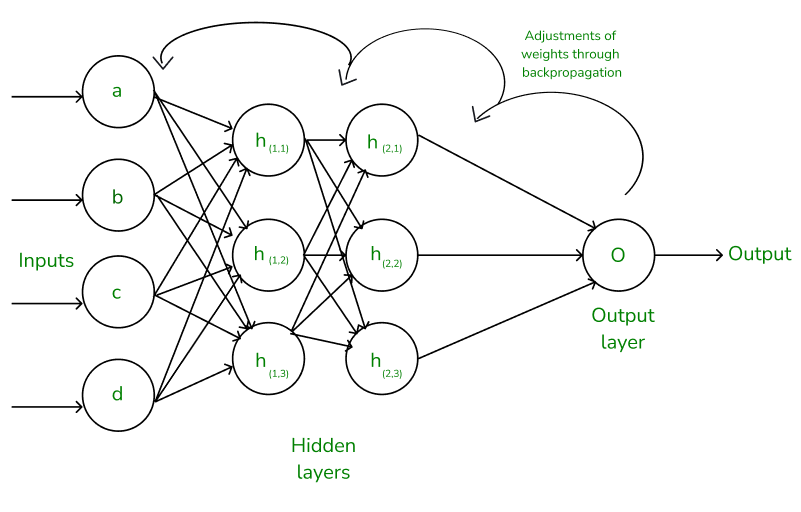
\includegraphics[width=0.5\textwidth]{Images/Frame-13.png}
    \caption{Diagrama ilustrativo del proceso de entrenamiento y retropropagación. \textit{Fuente: Imagen tomada de GeeksforGeeks, recuperada de \url{https://www.geeksforgeeks.org/backpropagation-in-neural-network/}.}}
    \label{fig:Backpropagaion}
\end{figure}

\vspace{7pt}
\subsubsection{iv. Tipos de Aprendizaje}
El \textit{Machine Learning} (ML) comprende un conjunto de técnicas y algoritmos que permiten a las máquinas aprender de los datos y realizar predicciones o tomar decisiones sin estar explícitamente programadas para cada tarea (\cite{elementosIA}). Una de las distinciones fundamentales dentro del ML se basa en el tipo de datos disponibles durante el entrenamiento, específicamente en si esos datos incluyen o no etiquetas o resultados esperados. De esta forma, se clasifican los enfoques de aprendizaje en cuatro categorías principales: \textbf{supervisado}, \textbf{no supervisado}, \textbf{semisupervisado} y \textbf{por refuerzo}.
\begin{itemize}
    \item \textbf{Aprendizaje Supervisado}: Este tipo de aprendizaje se basa en un conjunto de datos etiquetado, en el que cada instancia contiene características (\textit{features}) y un resultado conocido (\textit{target}) (\cite{choi2020introduction}). El objetivo es que el modelo aprenda una función de mapeo $f(x) = y$, $x$ representa las entradas y $y$ la salida esperada. Para dar un ejemplo, pensemos en una empresa inmobiliaria que busca predecir el precio de una casa según su número de habitaciones, area en metros cuadrados y ubicación puede utilizar aprendizaje supervisado entrenando un modelo con ejemplos historicos de ventas. El conjunto de datos se divide usualmente en subconjuntos de entrenamiento, validación y prueba, para ajustar, afinar y evualuar el modelo, respectivamente. Las tareas tipicas en este enfoque incluyen:
    \begin{itemize}
    \item\textbf{Regresión}: predicción de valores numéricos continuos (por ejemplo, precios de viviendas).
    \item\textbf{Clasificación}: predicción de categorias discretas (por ejemplo, rango de precios como (0-125k), (125-250k), etc.).    
    \end{itemize}
    \item \textbf{No Supervisado}: A diferencia del aprendizaje supervisado, este enfoque no cuenta con etiquetas o salidas conocidas asociadas a los datos. Es decir, el modelo no tiene una \textquotedblleft respuesta correcta\textquotedblright~que pueda utilizar como guia durante el entrenamiento. En su lugar, debe analizar los datos para identificar patrones subyacentes,estructuras o agrupaciones naturales presentes en ellos. El objetivo es encontrar representaciones útiles de los datos que permiten descubrir relaciones desconocidos o inferir características relevantes sin intervención humana directa (\cite{choi2020introduction}). \\[2pt]
    Este tipo de aprendizaje es especialmente útil en contextos donde obtener etiquetas es costoso y lento. En muchos casos de la vida real usando este metodo, como grandes bases de datos de clientes, imágenes, secuencias genéticas o registros médicos, se dispone de gran cantidad de informacíón sin clasificar, por lo que los algoritmos no supervisados resultan clave para el análisis exploratiorio y la extración automatica de conocimiento. \\[2pt]
    Las tareas más comunes dentro del aprendizaje no supervisado son:
    \begin{itemize}
        \item \textbf{Clustering (agrupamiento)}: agrupación de datos similares en clústeres basándose en sus características. Por ejemplo un algoritmo podría identificar subconjuntos de viviendas similares sin haber sido informado de categorías específicas.
        \item\textbf{Asociación}: descubrimiento de reglas o correlaciones frecuentes entre características. Útil para entender concurrencias comunes entre variables.
        \item\textbf{Detección de anomalías}: identificacíon de instancias atípicas o fuera de lo común, como precios de vivienda inusualmente altos en un vecindario.
    \end{itemize}
    Este tipo de aprendizaje es valioso cuando etiquetar datos resulta cosotoso o inviable, permitiendo extraer conocimiento directamente de la estructura de los datos.
\end{itemize}
\begin{figure}[H]
\centering
\begin{tikzpicture}[scale=0.8]
    % Supervised Learning (Izquierda)
    \begin{scope}[xshift=-6cm]
        % Ejes
        \draw[thick, ->] (0,0) -- (5,0);
        \draw[thick, ->] (0,0) -- (0,4);
        
        % Puntos rojos (clase 1)
        \foreach \x/\y in {0.5/0.8, 0.8/1.2, 1.2/0.6, 0.6/1.5, 1.0/1.8, 0.4/2.1, 0.9/2.3, 1.3/1.9, 0.7/2.7, 1.1/2.5}
            \fill[red] (\x,\y) circle (2pt);
        
        % Puntos azules (clase 2)
        \foreach \x/\y in {2.5/2.8, 2.8/3.2, 3.2/2.6, 2.6/3.5, 3.0/2.2, 2.4/2.4, 2.9/1.8, 3.3/2.1, 2.7/1.5, 3.1/1.9, 3.5/2.3, 3.8/2.7, 3.4/3.1, 2.2/3.0}
            \fill[blue] (\x,\y) circle (2pt);
        
        % Línea de decisión (discontinua)
        \draw[thick, dashed, black] (1.8,0.2) -- (2.2,3.8);
        
        % Título
        \node[below] at (2.5,-0.3) {\textbf{Supervised learning}};
    \end{scope}
    
    % Línea divisoria vertical
    \draw[thick] (0,-0.5) -- (0,4.5);
    
    % Unsupervised Learning (Derecha)
    \begin{scope}[xshift=1cm]
        % Ejes
        \draw[thick, ->] (0,0) -- (5,0);
        \draw[thick, ->] (0,0) -- (0,4);
        
        % Primer cluster (círculo izquierdo)
        \draw[thick, gray, dashed] (1.2,2.0) circle (0.8);
        \foreach \x/\y in {0.8/1.8, 1.0/2.2, 1.4/1.9, 1.3/2.3, 0.9/2.0, 1.5/2.1, 1.1/1.7, 1.6/1.8}
            \fill[gray] (\x,\y) circle (2pt);
        
        % Segundo cluster (círculo derecha-arriba)
        \draw[thick, gray, dashed] (3.5,3.0) circle (0.7);
        \foreach \x/\y in {3.2/2.8, 3.4/3.2, 3.8/2.9, 3.7/3.3, 3.3/3.0, 3.9/3.1, 3.5/2.7, 3.1/3.1}
            \fill[gray] (\x,\y) circle (2pt);
        
        % Tercer cluster (círculo derecha-abajo)
        \draw[thick, gray, dashed] (3.8,1.2) circle (0.6);
        \foreach \x/\y in {3.5/1.0, 3.7/1.4, 4.1/1.1, 4.0/1.5, 3.6/1.2, 4.2/1.3, 3.8/0.9}
            \fill[gray] (\x,\y) circle (2pt);
        
        % Puntos dispersos
        \foreach \x/\y in {0.5/0.5, 2.0/0.8, 4.3/2.2, 1.8/3.5}
            \fill[gray] (\x,\y) circle (2pt);
        
        % Título
        \node[below] at (2.5,-0.3) {\textbf{Unsupervised learning}};
    \end{scope}
\end{tikzpicture}

\caption{Ejemplo gráfico comparativo de algoritmos de aprendizaje supervisado y no supervisado.\textit{Fuente: Elaboración propia.}}
\label{fig:aprendizaje-supervisado-no-supervisado}
\vspace{2mm}

\small\textit{Nota:} En la parte izquierda (aprendizaje supervisado), la línea discontinua representa una frontera de decisión aprendida a partir de datos etiquetados. En cambio, el gráfico derecho (aprendizaje no supervisado) muestra cómo los algoritmos agrupan automáticamente los datos sin etiquetas previas, basándose únicamente en similitud o cercanía.

\end{figure}
\subsection{b. Nociones de Redes Neuronales (NN)}
\vspace{5pt}

\subsubsection{i.Componentes de la Red: Neuronas, Capas, Pesos,Activación} 
\vspace{3pt}
Las \textit{Redes Neuronales (NN)} son una clase de modelos matemáticos y computacionales diseñados para reconocer patrones y relaciones complejas entre datos (\cite{sanchez}). Se inspiran libremente en el funcionamiento del cerebro humano, particularmente en la forma en que las neuronas biológicas se comunican a través de sinapsis para procesar información.

En términos generales, una red neuronal está compuesta por un conjunto de unidades computacionales llamadas \textbf{neuronas artificiales}, organizadas en capas conectadas entre sí mediante enlaces ponderados. En nuestro contexto actual acerca del aprendizaje automático, las redes neuronales forman la base del \textbf{aprendizaje profundo} (\textit{Deep Learning}), especialmente cuando estas redes poseen múltiples capas.

\begin{itemize}
    \item\textbf{Neuronas}: son las unidades básicas de procesamiento de la red. Cada neurona recibe entradas numéricas, las combina mediante una operación de suma ponderada y aplica una función de activación para determinar su salida. Esta salida se propaga hacia las neuronas de la siguiente capa. Aunque una sola neurona tiene capacidad limitada, al ser organizadas en grandes conjuntos y capas interconectadas, adquieren una potencia por sí solas (\cite{datacamp_redes}).

    \item\textbf{Capas}:
    \begin{itemize}
        \item \textbf{Capa de entrada}: Corresponde a los datos que se introducen en la red. Cada nodo representa una característica del conjunto de datos( por ejemplo: color, tamaño,edad,etc.):
        \item\textbf{Capas ocultas}: Las capas ocultas de una red neuronal contienen unidades no observables y son las encargadas de transformar la información mediante operaciones sucesivas. En redes profundas (\textit{deep networks}), estas capas pueden ser numerosas, lo que permite modelar funciones altamente complejas.
        \item\textbf{Capa de salida}: Genera la predicción final del modelo, ya sea una clase, un valor numérico o una distribución de probabilidad, dependiendo del problema a resolver.
    \end{itemize}

   \item\textbf{Pesos y Sesgos (Biases)}:
    \begin{itemize}
        \item \textbf{Pesos}: Cada conexión entre neuronas tiene un peso asociado, que representa la fuerza o importancia de esa conexión. Durante el proceso de entrenamiento, estos pesos son ajustados iterativamente para que la red aprenda de los datos y reduzca su error en las predicciones.
        \item \textbf{Sesgos}: Son valores adicionales que se suman a la entrada de la función de activación de cada neurona. Actúan como un parámetro de ajuste adicional, permitiendo desplazar la salida de una neurona y mejorar la capacidad de aprendizaje del modelo.
    \end{itemize}
    \item \textbf{Funciones de Activación}: Estas funciones determinan la salida de cada neurona a partir de su entrada ponderada. Son importantes porque introducen no linealidades en el modelo, lo que nos permite que las redes neuronales aprendan relaciones complejas más allá de simples combinaciones lineales (\cite{datacamp_redes}). Algunas de las funciones de activación más comunes incluyen:
    \begin{itemize}
        \item \textbf{ReLU (Rectified Linear Unit)}: Devuelve cero si la entrada es negativa, y la entrada misma si es positiva. Es eficiente y muy utilizada en redes profundas.
        \item \textbf{Sigmoide}: Convierte las entradas en valores entre 0 y 1, útil en tareas de clasificación binaria. 
        \item \textbf{Tanh (Tangente Hiperbólica)}: Similar a la sigmoide pero con salida entre -1 y 1, centrada en cero, lo cual puede favorecer una convergencia más rápida durante el entrenamiento.
    \end{itemize}
\end{itemize}
\begin{figure}[H]
    \centering
    \begin{tikzpicture}[scale=1.5]
        % Nodos de entrada
        \draw (0,2) circle (0.2) node {$x_1$};
        \draw (0,1) circle (0.2) node {$x_2$};
        \draw (0,0) circle (0.2) node {$x_3$};
        
        % Nodos ocultos
        \draw (2,2) circle (0.2) node {$h_1$};
        \draw (2,1) circle (0.2) node {$h_2$};
        \draw (2,0) circle (0.2) node {$h_3$};
        
        % Nodo de salida
        \draw (4,1) circle (0.2) node {$y$};
        
        % Conexiones
        \draw (0.2,2) -- (1.8,2);
        \draw (0.2,2) -- (1.8,1);
        \draw (0.2,2) -- (1.8,0);
        \draw (0.2,1) -- (1.8,2);
        \draw (0.2,1) -- (1.8,1);
        \draw (0.2,1) -- (1.8,0);
        \draw (0.2,0) -- (1.8,2);
        \draw (0.2,0) -- (1.8,1);
        \draw (0.2,0) -- (1.8,0);
        
        \draw (2.2,2) -- (3.8,1);
        \draw (2.2,1) -- (3.8,1);
        \draw (2.2,0) -- (3.8,1);
        
        % Etiquetas
        \node at (0,2.5) {Entrada};
        \node at (2,2.5) {Oculta};
        \node at (4,1.5) {Salida};
    \end{tikzpicture}
\caption{Estructura típica de una red neuronal, que incluye la capa de entrada, varias capas ocultas y la capa de salida. \textit{Fuente: Elaboración propia.}}
    \label{fig:red-neuronal-tikz}
\end{figure}
Ver Anexo A para información complementaria.
\subsubsection{ii. Inferencia por propagación hacia adelante}
La propagación hacia adelante (\textit{forward propagation}) es el proceso por el que una red neuronal transforma los datos de entrada en predicciones o salidas (\cite{datacamp_redes}). En términos técnicos, es el cálculo secuencial que mueve los datos desde la capa de entrada, a través de las capas ocultas y, finalmente, a la capa de salida (\cite{nvidia}). Durante este recorrido, los datos se transforman mediante conexiones ponderadas y funciones de activación, lo que permite a la red captar patrones complejos. \\
La importancia de la propagación hacia adelante radica en que es el mecanismo principal por el cual el modelo genera sus predicciones basadas en los parámetros que ha aprendido durante el entrenamiento que se le da. Sin este proceso, no sería posible evaluar cómo se comporta la red ante nuevos datos sin medir su desempeño. Además, la propagación hacia adelante es esencial para calcular la función de pérdida, que es la medición de los errores entre las predicciones y los valores reales. Esta información es usada posteriormente durante la retropropagación  para ajustar los pesos de la red y mejorar su precisión. Para más detalles, consulte el Anexo A.
\begin{figure}[H]
    \centering
    \scalebox{0.8}{
    \begin{tikzpicture}[
        neuron/.style={circle, draw=black, fill=blue!20, minimum size=12mm},
        arrow/.style={-{Stealth[length=3mm, width=2mm]}, thick, blue},
        layerlabel/.style={font=\bfseries, align=center}
    ]

    % Capas
    % Capa Entrada
    \node[layerlabel] (inputlabel) at (0,4) {Entrada};
    \node[neuron] (I1) at (0,3) {$x_1$};
    \node[neuron] (I2) at (0,2) {$x_2$};
    \node[neuron] (I3) at (0,1) {$x_3$};

    % Capa Oculta
    \node[layerlabel] (hiddenlabel) at (5,5) {Oculta};
    \node[neuron] (H1) at (5,3.5) {$h_1$};
    \node[neuron] (H2) at (5,2.5) {$h_2$};
    \node[neuron] (H3) at (5,1.5) {$h_3$};

    % Capa Salida
    \node[layerlabel] (outputlabel) at (10,3) {Salida};
    \node[neuron] (O1) at (10,2) {$y$};

    % Conexiones Entrada -> Oculta
    \draw[arrow] (I1) -- (H1);
    \draw[arrow] (I1) -- (H2);
    \draw[arrow] (I1) -- (H3);

    \draw[arrow] (I2) -- (H1);
    \draw[arrow] (I2) -- (H2);
    \draw[arrow] (I2) -- (H3);

    \draw[arrow] (I3) -- (H1);
    \draw[arrow] (I3) -- (H2);
    \draw[arrow] (I3) -- (H3);

    % Conexiones Oculta -> Salida
    \draw[arrow] (H1) -- (O1);
    \draw[arrow] (H2) -- (O1);
    \draw[arrow] (H3) -- (O1);


    \end{tikzpicture}
    }
    \caption{Propagación hacia adelante (Forward propagation) en una red neuronal simple.\textit{Fuente: Elaboración propia}}
    \label{fig:forward_propagation}
\end{figure}

\subsubsection{iii. Entrenamiento}
\vspace{3pt}
El entrenamiento de una red neuronal es un proceso donde ajustamos los pesos internos de la red con el fin de minimizar la diferencia entre las predicciones de la red y los valores reales esperados. Este proceso permite que la red aprenda a representar patrones presentes en los datos, generalizando su conocimiento para realizar predicciones sobre datos no vistos (\cite{zhou2020graph}). El entrenamiento está compuesto por dos fases principales: la evaluación del error, por medio de una \textbf{función de pérdida}, y la \textbf{actualización de los pesos} usando el algoritmo de \textit{propagación hacia atrás} (\textit{backpropagation}) (\cite{nvidia}).
\begin{itemize}
\item\textbf{1. Función de pérdida}:\newline
Es una función de pérdida cuantificada para saber qué tan bien o mal está funcionando una red. Calcula la diferencia entre la salida predicha por la red y el valor real esperado (\cite{zhou2020graph}). El objetivo del entrenamiento es minimizar esta función de perdida mediante la actualización iterativa de los pesos. \newline Algunas funciones comunes son:
\begin{itemize}
    \item \textbf{Error cuadrático medio (MSE)}: Utilizada en tareas de regresión, se define como : $\mathcal{L}_{MSE} = \frac{1}{n} \sum_{i=1}^{n}(y_i - \hat{y}_i)^2$
    \item \textbf{Entropía cruzada}: Utilizada para clasificación, especialmente con salidas probabilísticas. Si se tiene una salida verdadera $y$ y una predicción $\hat{y}$, la pérdida es: $\mathcal{L}_{CE} = -\sum y \log(\hat{y})$
\end{itemize}

\item\textbf{2. Propagación hacia atrás (Backpropagation)}:\newline
Este es un algoritmo central para entrenar redes neuronales. Utiliza el cálculo de derivadas (gradientes) para actualizar los pesos de la red en dirección contraria a la propagación hacia adelante . El proceso sigue los siguientes pasos:
\begin{enumerate}
    \item Se realiza una propagación hacia adelante para obtener las predicciones.
    \item Se calcula la pérdida comparando con los valores reales.
    \item Se aplica la regla de la cadena para propagar el error desde la capa de salida hacia atrás, capa por capa, computando los gradientes parciales con respecto a cada peso.
    \item Se actualizan los pesos mediante un algoritmo de optimización, típicamente descenso del gradiente:$w \leftarrow w - \eta \cdot \frac{\partial \mathcal{L}}{\partial w}$, donde $\eta$ es la tasa de aprendizaje.
\end{enumerate}
Este proceso se repite en multiples iteraciones (\textit{epochs}) sobre el conjunto de entrenamiento. Al finalizar, la red ha ajustado sus parámetros internos para producir predicciones más precisas.

\item \textbf{Regularización y generalización}: \newline
Para evitar el sobreajuste (overfitting), es común introducir técnicas de regularización como \textit{Dropout}, \textit{L2 regulization}, o el uso de validación cruzada. Estas técnicas mejoran la capacidad de generalización del modelo.
\end{itemize}
\begin{figure}[H]
    \centering
    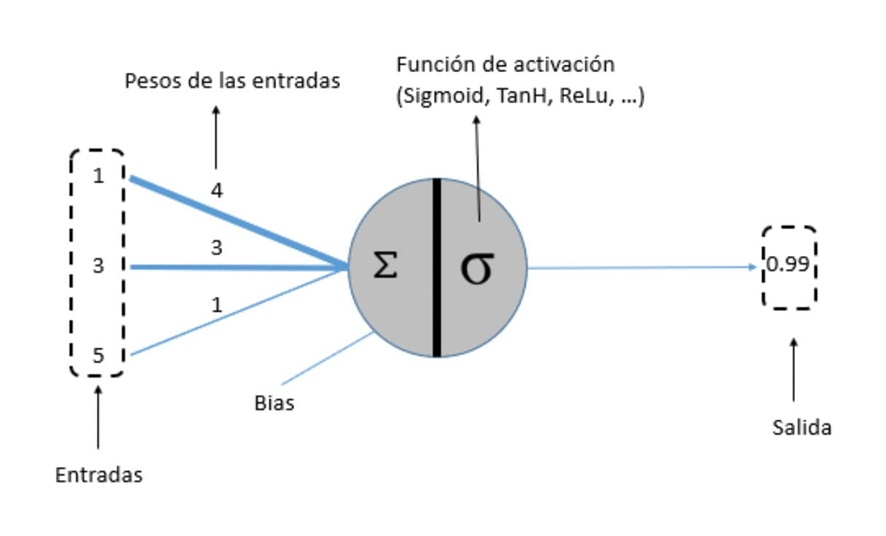
\includegraphics[width=0.5\textwidth]{Images/111-1.jpg}
    \caption{Modelo de una neurona artificial. Cada entrada es multiplicada por un peso, se suma un sesgo (bias) y se aplica una función de activación (como Sigmoid, Tanh o ReLU) para obtener la salida. \textit{Fuente: Imagen tomada de Ángel Villazón, recuperada de \url{https://www.angelvillazon.com/inteligencia-artificial-robotica/entrenamiento-de-redes-neuronales/}.}}
    \label{fig:neurona-artificial}
\end{figure}

\subsection{c. Aplicaciones} 
\vspace{3pt}
Las redes neuronales tienen un amplio uso de aplicaciones practicas que abarcan desde el análisis de imágenes hasta el procesamiento de lenguaje natural (\cite{hui2021gnn}). Estás aplicaciones aprovechan la capacidad de las redes para aprender representaciones complejas y generalizar a partir de datos de entrenamiento en diferentes contextos del mundo real.
\begin{itemize}
\item \textbf{i. Reconocimiento de Imágenes}; \newline
Las redes neuronales de grafos (GNN) han ampliado las posibilidades en el reconocimiento de imágenes, especialmente cuando estas se representan como grafos, como en el caso de imágenes con superpíxeles o estructuras espaciales irregulares. Permiten tareas como clasificación de objetos, detección de patrones, segmentación y reconocimiento de escritura manuscrita a partir de representaciones gráficas (\cite{hui2021gnn}). Estas redes son capaces de extraer automáticamente características relevantes mediante el intercambio de información entre nodos conectados, lo cual reduce la necesidad de ingeniería manual de características. Se aplican en visión por computadora basada en grafos, diagnóstico médico (analizando relaciones espaciales en imágenes), vehículos autónomos (procesamiento estructural de escenas), y sistemas inteligentes de vigilancia.


    \item \textbf{ii. Procesamiento de Lenguaje Natural (NLP)}: \newline
    En el campo del procesamiento del lenguaje natural, las redes neuronales han hecho posibles avances significativos gracias a arquitecturas como RNN, LSTM y los modelos de transformadores (\cite{aws2025nlp}). Estas arquitecturas permiten capturar la estructura y semántica del lenguaje humano, facilitando tareas como traducción automática, análisis de sentimientos, generación de texto, respuesta a preguntas, detección de spam, y clasificación de documentos.
    

\end{itemize}
\newpage
{\section{Fundamentos y justificación de GNNs}} 
\vspace{5pt}
Las \textbf{Redes neuronales de Grafos} (GNNs, por sus siglas en inglés) son una clase de modelos diseñados específicamente para trabajar con datos estructurados como grafos (\cite{hui2021gnn}). Estos modelos extienden la capacidad de las redes neuronales tradicionales al considerar explícitamente la estructura de conexiones entre elementos, permitiendo aprender representaciones útiles de nodos, aristas y del grafo completo. Se han vuelto fundamentales en tareas que involucran relaciones complejas, como redes sociales, conocimiento biomecular, sistemas de recomendación, y más. Para más detalles, consulte el Anexo B.
\vspace{3pt}
\subsection{a. Definiciones Básicas} 
Un \textbf{grafo} $G = (V, E)$ está compuesto por un conjunto de nodos (vértices) $V$ y un conjunto de aristas (enlaces) $E \subseteq V \times V$. En muchos contextos, tanto los nodos como las aristas están asociados a vectores de características. Por ejemplo, en un grafo de usuarios, cada nodo puede representar a un usuario con atributos como edad, ubicación e intereses, y cada arista puede representar una amistad o interacción.
\begin{figure}[h]
\centering
\begin{tikzpicture}[scale=1.2]

% Nodos simples
\node[circle, draw, fill=blue!20, minimum size=12mm] (A) at (0, 2) {Ana};
\node[circle, draw, fill=green!20, minimum size=12mm] (B) at (3, 3) {Carlos};
\node[circle, draw, fill=yellow!20, minimum size=12mm] (C) at (3, 1) {Luis};
\node[circle, draw, fill=pink!20, minimum size=12mm] (D) at (6, 2) {María};

% Aristas simples
\draw[thick] (A) -- (B) node[midway, above] {Amigos};
\draw[thick] (A) -- (C) node[midway, left] {Trabajo};
\draw[thick] (B) -- (D) node[midway, above] {Pareja};
\draw[thick] (C) -- (D) node[midway, below] {Vecinos};

% Etiquetas
\node at (3, 0) {$G = (V, E)$};
\node at (3, -0.5) {$V = \{Ana, Carlos, Luis, Maria\}$};

\end{tikzpicture}
\caption{Ejemplo grafo simple de usuarios.\textit{Fuente: Elaboración propia.}}
\label{fig:grafo_simple}
\end{figure}

\subsection{b. Limitaciones de las Redes Neuronales Convencionales para Grafos}
\vspace{3pt}
Las redes neuronales tradicionales, como las redes densas (fully connected) o convolucionales (CNN), están diseñadas para entradas con estructuras regulares: vectores de tamaño fijo, imágenes en forma de grillas o secuencias ordenadas (\cite{adrformacion2025}). Sin embargo, estas arquitecturas presentan dificultades al aplicarse directamente sobre grafos, los cuales poseen características estructurales propias que desafían dichos modelos. A continuación se detallan algunas limitaciones clave:


\begin{itemize}
    \item \textbf{Estructura irregular}: A diferencia de las imágenes, donde cada píxel tiene un número fijo y ordenado de vecinos, los nodos en un grafo pueden tener un número arbitrario y variable de conexiones. Esto dificulta el uso de operaciones estándar de convolución o agrupación.

    \item \textbf{Invarianza a permutaciones}: El significado de un grafo no depende del orden en que se listan sus nodos o aristas, pero las redes tradicionales tienden a aprender patrones sensibles al orden de los datos. Esta falta de invarianza puede llevar a que el modelo no generalice bien.

    \item \textbf{Dependencias de largo alcance}: Muchas relaciones importantes en un grafo ocurren entre nodos que no están directamente conectados. Las arquitecturas tradicionales tienen dificultades para capturar tales relaciones sin un mecanismo de propagación específico.

    \item \textbf{Escalabilidad y eficiencia}: Aplicar modelos tradicionales directamente sobre representaciones matriciales del grafo (como la matriz de adyacencia) puede ser computacionalmente costoso en grafos grandes o dinámicos, lo cual limita su aplicabilidad práctica en escenarios del mundo real.
\end{itemize}

Estas limitaciones motivaron el desarrollo de arquitecturas especializadas como las GNNs, que permiten incorporar la topología del grafo en el proceso de aprendizaje de manera eficiente y flexible.

\subsection{c. Tipos y usos de GNNs}
\vspace{3pt}
Con el fin de superar las limitaciones estructurales que presentan los grafos para arquitecturas tradicionales, se han propuesto diversas variantes de redes neuronales de grafos. A continuación se describen tres de las más representativas:
    
\subsubsection{i. Graph Convolutional Networks (GCNs)}
Las GCNs extienden la operación de convolución a grafos, utilizando una matriz de adyacencia normalizada para propagar información entre nodos. Cada nodo actualiza su representación combinando sus características con las de sus vecinos. Este enfoque ha sido ampliamente aplicado en tareas como la clasificación de nodos, la predicción de enlaces y la detección de comunidades. No obstante, su capacidad se ve limitada por el problema del \textit{oversmoothing}, que ocurre cuando muchas capas hacen que las representaciones de los nodos se vuelvan demasiado similares (\cite{kipf2016semi}). ver más en Anexo B.

\subsubsection{ii. Graph Attention Networks (GATs)}
Las GATs incorporan un mecanismo de atención que permite a cada nodo ponderar de forma diferenciada la información proveniente de sus vecinos. A través de coeficientes de atención aprendibles, el modelo decide qué nodos vecinos son más relevantes para la actualización del estado del nodo central. Este enfoque ha demostrado ventajas en grafos con relaciones heterogéneas o asimétricas, como los de conocimiento o redes sociales (\cite{dgl2024gat}).

\subsubsection{iii. GraphSAGE (Graph Sample and Aggregate)}
GraphSAGE es un modelo inductivo que permite generalizar a nodos no vistos durante el entrenamiento. Esto se logra mediante el muestreo de un subconjunto fijo de vecinos y el uso de funciones de agregación (como media, suma o max-pooling). Es especialmente adecuado para grafos de gran escala o dinámicos, como los utilizados en motores de recomendación, análisis de tráfico y monitoreo de redes de sensores.

\begin{figure}[H]
\centering
\begin{tikzpicture}[
    node/.style={circle, draw, minimum size=0.8cm, font=\scriptsize},
    edge/.style={->, >=stealth},
    hidden/.style={rectangle, draw, minimum size=0.3cm, fill=yellow!30}
]

% Título
\node[font=\small\bfseries] at (0, 5) {Ejemplo de Graph Attention Network (GAT)};

% Nodos de entrada (lado izquierdo)
\node[node, fill=blue!40] (h0) at (-3, 3.5) {$h_0$};
\node[node, fill=blue!40] (h1) at (-3, 2.5) {$h_1$};
\node[node, fill=blue!40] (h2) at (-3, 1.5) {$h_2$};
\node[node, fill=blue!40] (h3) at (-3, 0.5) {$h_3$};
\node[node, fill=blue!40] (h4) at (-3, -0.5) {$h_4$};

% Capa oculta (amarillo)
\draw[fill=yellow!20, draw] (-1.3, -1) rectangle (-0.7, 4.5);
\node[font=\tiny, rotate=90] at (-1, 1.75) {Mecanismo de Atención};

% Nodo objetivo
\node[node, fill=orange!50] (target) at (1, 2) {$e_1$};

% Función Softmax
\node[circle, draw, minimum size=1cm, fill=pink!30] (softmax) at (3, 2) {\scriptsize Softmax};

% Coeficientes de atención (salida)
\node[node, fill=red!40] (a10) at (5, 3.5) {$\alpha_{10}$};
\node[node, fill=red!40] (a11) at (5, 2.8) {$\alpha_{11}$};
\node[node, fill=red!40] (a12) at (5, 2.1) {$\alpha_{12}$};
\node[node, fill=red!40] (a13) at (5, 1.4) {$\alpha_{13}$};
\node[node, fill=red!40] (a14) at (5, 0.7) {$\alpha_{14}$};

% Conexiones de entrada al mecanismo de atención
\draw[edge] (h0) -- (-1, 3.5);
\draw[edge] (h1) -- (-1, 2.8);
\draw[edge] (h2) -- (-1, 2.1);
\draw[edge] (h3) -- (-1, 1.4);
\draw[edge] (h4) -- (-1, 0.7);

% Del mecanismo de atención al nodo objetivo
\draw[edge] (-0.7, 2) -- (target);

% Del nodo objetivo al softmax
\draw[edge] (target) -- (softmax);

% Del softmax a los coeficientes
\draw[edge] (softmax) -- (a10);
\draw[edge] (softmax) -- (a11);
\draw[edge] (softmax) -- (a12);
\draw[edge] (softmax) -- (a13);
\draw[edge] (softmax) -- (a14);

% Etiquetas explicativas
\node[font=\tiny] at (-3, 4.2) {Características de nodos};
\node[font=\tiny] at (1, 1.3) {Scores de atención};
\node[font=\tiny] at (5, 4.2) {Coeficiente normalizados};

\end{tikzpicture}
\caption{Ejemplo del mecanismo de atención en Graph Attention Networks (GAT). El modelo calcula scores de atención $e_{ij}$ entre nodos, los normaliza usando softmax para obtener coeficientes $\alpha_{ij}$, y luego pondera las características de los nodos vecinos según su relevancia. Fuente: Adaptado de \textit{Understand Graph Attention Network — DGL 2.0.0 documentation}.}
\label{fig:gat_example}
\end{figure}
\newpage 
\section{Caso de Estudio GCN} \vspace{10pt}

\subsection{a. Definición y Justificación}

Una Red Convolucional sobre Grafos (GCN, por sus siglas en inglés) es un tipo de red neuronal diseñada para trabajar directamente con estructuras en forma de grafo. A diferencia de las redes tradicionales, que esperan como entrada datos organizados en forma de vectores o matrices (como las imágenes o secuencias), las GCN pueden procesar datos cuya forma natural es un conjunto de nodos conectados por relaciones, como ocurre en redes sociales, mapas de relaciones científicas o redes biológicas (\cite{zhou2020graph, bronstein2017geometric}).

Las GCN fueron propuestas por Thomas Kipf y Max Welling en 2016 (\cite{kipf2016semi}), como una solución para tareas como la clasificación de nodos dentro de un grafo, especialmente en situaciones donde no todos los nodos tienen etiquetas conocidas. Lo innovador de este modelo es que puede aprender a predecir etiquetas utilizando tanto las características de cada nodo como la estructura de conexiones entre ellos, sin necesidad de transformar el grafo en una estructura lineal.

Esto es especialmente útil en problemas donde solo se conoce la clase o etiqueta de algunos pocos nodos, ya que la GCN puede aprovechar las conexiones del grafo para extender esa información a los demás nodos. Además, las GCN permiten realizar este proceso de forma eficiente, utilizando operaciones simples pero efectivas que se pueden aplicar directamente sobre la estructura del grafo.
\subsection{b. Características Distintivas}

Las GCN tienen varias propiedades clave que las hacen diferentes a otros modelos de aprendizaje automático (\cite{wu2020comprehensive}). A continuación se explican junto con un ejemplo ilustrativo basado en una red de recomendación de películas:

\begin{itemize}
    \item \textbf{Agregación de información local:} en cada capa, un nodo combina su información con la de sus vecinos directos. Por ejemplo, si una persona no ha indicado sus gustos de películas, pero sus amigos sí lo han hecho, se puede usar esa información para inferir qué películas le podrían gustar.

    \item \textbf{Uso de los mismos parámetros:} la misma matriz de pesos se aplica a todos los nodos. Esto permite detectar patrones similares en distintas partes del grafo. En nuestro ejemplo, sin importar si un nodo representa a “Ana” o “Luis”, el modelo usa los mismos parámetros para actualizar su representación.

    \item \textbf{Independencia del orden de los vecinos:} como el orden de los amigos no afecta a quién me influye más o menos, las operaciones como el promedio son ideales para que el modelo funcione sin importar cómo estén ordenados los vecinos.

    \item \textbf{Generalización a distintos grafos:} una GCN puede usarse en grafos con estructuras diferentes. Por ejemplo, si se entrena en una red de usuarios de una ciudad, puede aplicarse luego a otra red de usuarios de otra ciudad que tengan conexiones y gustos similares.
\end{itemize}

\begin{figure}[H]
    \centering
    \begin{tikzpicture}[every node/.style={circle, draw, minimum size=1cm}, node distance=2cm]
        \node[fill=yellow!30] (A) at (0,0) {¿?};
        \node[fill=blue!20] (B) at (-2,1.5) {Si};
        \node[fill=blue!20] (C) at (2,1.5) {Si};
        \node[fill=blue!20] (D) at (-2,-1.5) {Si};
        \node[fill=red!20] (E) at (2,-1.5) {No};

        \draw (A) -- (B);
        \draw (A) -- (C);
        \draw (A) -- (D);
        \draw (A) -- (E);
    \end{tikzpicture}
    \caption{Ejemplo de GCN en una red de recomendación. El nodo central no tiene información directa, pero puede inferirse por los gustos de sus amigos (Si = le gusta el cine, No = no le gusta) \textit{Fuente: Elaboración propia}.}
    \label{fig:movie_recommendation}
\end{figure}

\vspace{0.5em}
En la Figura, el nodo central representa a una persona la cual se desconoce su gusto por el cine (¿?). Sin embargo, tres de sus amigos ya indicaron que les gusta el cine, y uno que no. Gracias a la GCN, el nodo puede actualizar su representación combinando estas señales y así predecir si probablemente también le gusten las películas.




\subsection{c. Modelo de Propagación}

El modelo de propagación define cómo se actualizan las representaciones de los nodos usando tanto sus características como las conexiones en el grafo (\cite{kipf2016semi, hamilton2017inductive}).

\subsubsection{i. Features}

Cada nodo $i$ tiene un vector de características $\mathbf{x}_i \in \mathbb{R}^F$, donde $F$ es el número de atributos que describen ese nodo. Por ejemplo, en un grafo de artículos científicos como Cora, estos atributos pueden indicar qué palabras aparecen en cada artículo.

Si hay $N$ nodos, se puede representar toda la información en una sola matriz $X \in \mathbb{R}^{N \times F}$, donde cada fila corresponde a un nodo y cada columna a una característica.

\subsubsection{ii. Matriz de Adyacencia}

La \textit{matriz de adyacencia}, denotada como $A \in \mathbb{R}^{N \times N}$. Esta matriz tiene un valor $A_{ij} = 1$ si existe una conexión directa (una arista) entre el nodo $i$ y el nodo $j$, y un valor $A_{ij} = 0$ si no hay conexión.

Sin embargo, en el modelo GCN también se quiere que cada nodo tenga en cuenta su propia información al actualizarse. Para lograr esto, se agregan conexiones del nodo consigo mismo, llamadas \textit{autoconexiones} o \textit{self-loops}. Esto se hace sumando la matriz identidad $I_N$ a la matriz de adyacencia original:

\[
\hat{A} = A + I_N
\]

Esta nueva matriz $\hat{A}$ se utiliza en los cálculos posteriores para la propagación de información.


\subsubsection{iii. Matriz de Pesos}

La \textit{matriz de pesos}, denotada como $W^{(l)}$, se utiliza para transformar las representaciones de los nodos en cada capa $l$ de la GCN. Esta transformación es lineal y permite que el modelo aprenda a combinar y proyectar las características de los nodos a un nuevo espacio de representación.

Cada capa tiene su propia matriz de pesos, que se ajusta automáticamente durante el entrenamiento. Esta matriz actúa sobre la información agregada de los vecinos y del propio nodo, permitiendo capturar patrones útiles para la tarea de aprendizaje.

La fórmula general para calcular la salida de una capa es:

\[
H^{(l+1)} = \sigma\left( \hat{D}^{-1/2} \hat{A} \hat{D}^{-1/2} H^{(l)} W^{(l)} \right)
\]

donde:
\begin{itemize}
    \item $H^{(0)} = X$, la matriz de características iniciales de los nodos,
    \item $\hat{A}$ es la matriz de adyacencia con autoconexiones,
    \item $\hat{D}$ es la matriz diagonal de grados asociada a $\hat{A}$,
    \item $\sigma$ es una función de activación no lineal.
\end{itemize}

\subsubsection{iv. Normalización y Activación}

El término $\hat{D}^{-1/2} \hat{A} \hat{D}^{-1/2}$ realiza una \textit{normalización simétrica} sobre la matriz de adyacencia modificada $\hat{A}$. Esta normalización ajusta los valores de las conexiones en función del grado de los nodos, es decir, del número total de conexiones que tiene cada nodo, incluyendo las autoconexiones.

Para construir la matriz $\hat{D}$, se calcula la suma de cada fila de $\hat{A}$ y se coloca ese valor en la diagonal correspondiente. De esta forma, $\hat{D}_{ii} = \sum_j \hat{A}_{ij}$. El objetivo de esta normalización es evitar que los nodos con muchos vecinos dominen el proceso de agregación, manteniendo un equilibrio entre la influencia de todos los nodos.

La función $\sigma$ representa una activación no lineal que se aplica después de la agregación y la transformación lineal. En las capas ocultas se suele usar la función ReLU, que introduce no linealidad al modelo. En la capa final, si el problema es de clasificación, se utiliza la función softmax para obtener una distribución de probabilidades sobre las posibles clases. Ver Anexo C para información complementaria.

\subsection{d. Agregación de Features y Transformación de Nodos}

En cada capa de una GCN, los nodos actualizan sus representaciones combinando sus propias características con las de sus vecinos. Este proceso se conoce como \textit{agregación de features}. A medida que el modelo avanza por las capas, cada nodo puede acceder a información de vecinos más lejanos dentro del grafo.

La representación del nodo $v$ en la capa $l+1$ se calcula como:

\[
\mathbf{h}_v^{(l+1)} = \sigma \left( \sum_{u \in \mathcal{N}(v) \cup \{v\}} \frac{1}{\sqrt{d_v d_u}} \mathbf{h}_u^{(l)} W^{(l)} \right)
\]

donde $\mathcal{N}(v)$ es el conjunto de vecinos del nodo $v$, y $d_v$ es su grado (incluyendo la autoconexión). En esta fórmula, cada nodo combina las representaciones de sus vecinos y las suyas propias, las transforma linealmente con $W^{(l)}$, y aplica una función de activación.

Este proceso se repite en múltiples capas. Con cada nueva capa, el nodo incorpora información de una vecindad más amplia, lo que permite construir una representación final que refleja tanto sus atributos individuales como la estructura del grafo a su alrededor.


\subsection{e. Aplicaciones}

\subsubsection{i. Redes Sociales}

Las GCN se han utilizado exitosamente en dominios como redes sociales, biología computacional y sistemas de recomendación (\cite{zhou2020graph}). Por ejemplo, en redes sociales es común aplicar GCNs para tareas como la predicción de intereses, la detección de comunidades o la recomendación de contenido.

Una aplicación frecuente es la \textit{clasificación de usuarios}, donde se busca predecir intereses, grupos a los que pertenece una persona o su probabilidad de interactuar con ciertos contenidos. Las GCN permiten usar no solo los datos directos de cada usuario (como su edad, gustos o historial de publicaciones), sino también la información de sus conexiones en la red, es decir, lo que hacen y comparten sus amigos o contactos cercanos. Esto es muy útil en casos donde el usuario no ha dado mucha información, ya que el modelo puede aprender a partir del comportamiento de su entorno.

Por ejemplo, si una persona sigue a varias cuentas relacionadas con deportes, aunque no lo haya indicado directamente, el modelo puede predecir que le interesan esos temas. Esto permite personalizar recomendaciones de forma más precisa, incluso con poca información inicial.

Además de la clasificación, las GCN también se usan en tareas como:

\begin{itemize}
    \item \textbf{Detección de comunidades:} identificar grupos de usuarios que están muy conectados entre sí y comparten características o comportamientos similares. Esto es útil, por ejemplo, para analizar la dinámica de grupos dentro de una red social o para estudiar cómo se propagan ideas o contenidos.
    
    \item \textbf{Predicción de vínculos:} anticipar la aparición de nuevas conexiones entre usuarios, como sugerencias de amistad o seguidores recomendados. El modelo aprende a reconocer patrones en las relaciones existentes y puede predecir cuáles usuarios probablemente se conecten en el futuro.
    
    \item \textbf{Filtrado de contenido:} estimar qué publicaciones o elementos serán relevantes para cada usuario, basándose no solo en su historial, sino también en cómo interactúan otros usuarios similares. Esto mejora la experiencia al mostrar contenido más ajustado a los intereses reales del usuario.
\end{itemize}

Estas aplicaciones muestran cómo las GCN aprovechan tanto la información individual como la estructura de la red para hacer predicciones más completas y precisas. Gracias a esto, se han convertido en una herramienta valiosa para plataformas digitales que necesitan entender mejor a sus usuarios y cómo se relacionan entre sí. Ver Anexo C para información complementaria.


\begin{figure}[H]
    \centering
    \begin{tikzpicture}[every node/.style={circle, draw, minimum size=1cm}, node distance=2cm]

        \node[fill=yellow!30] (A) at (-2,0) {A};
        \node[fill=yellow!30] (B) at (2,0) {B};

        \node[fill=blue!20] (A1) at (-4,1.5) {};
        \node[fill=blue!20] (A2) at (-4,0) {};
        \node[fill=blue!20] (A3) at (-4,-1.5) {};

        \node[fill=blue!20] (B1) at (4,1.5) {};
        \node[fill=blue!20] (B2) at (4,0) {};
        \node[fill=blue!20] (B3) at (4,-1.5) {};

        \draw (A) -- (A1);
        \draw (A) -- (A2);
        \draw (A) -- (A3);

        \draw (B) -- (B1);
        \draw (B) -- (B2);
        \draw (B) -- (B3);

        \draw[dashed, thick] (A) -- (B);

    \end{tikzpicture}
    \caption*{Fuente: Creacion propia}
    \vspace{0.5em}
\end{figure}


\vspace{0.5em}
Ejemplo de predicción de vínculos. Aunque los usuarios A y B no están conectados directamente, sus redes de vecinos tienen una estructura muy parecida: ambos están conectados con otros nodos que tienen características similares en cantidad y patrón de conexión. Este tipo de similitud estructural puede ser detectada por una GCN al analizar las relaciones dentro del grafo.

Gracias al proceso de propagación de información entre nodos, la GCN es capaz de notar que A y B tienen contextos parecidos, aunque no compartan un vínculo en el presente. A partir de esto, el modelo puede predecir que existe una alta probabilidad de que se genere una conexión entre ellos en el futuro, como podría ocurrir en una red social donde se recomienda amistad o seguimiento entre usuarios con intereses y contactos comunes.

Este tipo de tarea es conocida como \textit{link prediction} y es muy útil, por ejemplo, para sugerencias de amistad en plataformas como Facebook o LinkedIn, donde se aprovechan patrones en la red de conexiones para anticipar nuevas relaciones.

\begin{figure}[H]
\centering
\begin{tikzpicture}[
    user/.style={circle, draw, fill=yellow!40, minimum size=1cm},
    post/.style={rectangle, draw, fill=blue!20, minimum size=0.8cm},
    edge/.style={thick},
    scale=1
]

% Usuario
\node[user] (U) at (0,0) {Usuario};

% Publicaciones vistas
\node[post] (P1) at (-3,1.5) {Post A};
\node[post] (P2) at (-3,0) {Post B};
\node[post] (P3) at (-3,-1.5) {Post C};

% Publicaciones no vistas
\node[post] (P4) at (3,1) {Post D};
\node[post] (P5) at (3,-1) {Post E};

% Conexiones usuario - publicaciones vistas
\draw[edge] (U) -- (P1);
\draw[edge] (U) -- (P2);
\draw[edge] (U) -- (P3);

% Conexiones entre posts (relaciones de contenido)
\draw[dashed] (P1) -- (P4);
\draw[dashed] (P2) -- (P4);
\draw[dashed] (P3) -- (P5);

\end{tikzpicture}
\caption{Ejemplo de filtrado de contenido con GCN. Fuente: Creación propia}
\label{fig:filtrado-contenido}
\end{figure}

Este ejemplo muestra cómo una GCN puede recomendar contenido a un usuario basándose en sus interacciones anteriores. Aunque el usuario no ha visto las publicaciones D y E, el modelo detecta que están relacionadas con otras que sí ha visto, y puede predecir que también serán de su interés. Este enfoque se usa comúnmente en sistemas de recomendación personalizados.





\newpage
\section{Ejemplo Demostrativo de GCN}
\vspace{10pt}

\subsection{a. Descripción del Problema (Clasificación de Nodos)} 
En esta demostración se utiliza el dataset \textit{Zachary’s Karate Club}, un conjunto de datos clásico en el análisis de grafos y redes sociales. Este dataset representa la estructura social de un club de karate universitario que, tras un conflicto interno, se dividió en dos grupos: aquellos que permanecieron con el administrador del club, conocido como \textit{Mr. Hi}, y aquellos que se alinearon con otro miembro llamado \textit{John A.} (\textit{Officer}).

Cada nodo en el grafo representa a un miembro del club, mientras que cada arista representa una relación de amistad entre dos miembros. El objetivo es realizar una clasificación de nodos, es decir, predecir a qué grupo (Mr. Hi u Officer) pertenece cada persona únicamente a partir de la estructura del grafo (las conexiones entre los miembros).

Para ello, se emplea una \textbf{Red Neuronal Convolucional sobre Grafos (GCN)}. Esta GCN toma como entrada la estructura del grafo y propaga características entre los nodos mediante las aristas, permitiendo inferir correctamente la etiqueta de cada nodo.

\subsection{b. Obtención del Dataset}
Este dataset está incluido en la librería de Python \texttt{NetworkX}, la cual se encuentra preinstalada en distribuciones como Anaconda. En caso de ser necesario, se puede instalar con el comando:

\begin{verbatim}
pip install networkx[default]
\end{verbatim}

\subsection{c. Configuración de la GCN}
Para implementar este modelo se requiere instalar las librerías \texttt{networkx}, \texttt{torch}, \texttt{collections} y \texttt{matplotlib} mediante:

\begin{verbatim}
pip install networkx matplotlib torch
\end{verbatim}

Una vez instaladas, se importa el grafo del dataset y se almacena como variable. También se obtiene el número de nodos (34 en este caso). Luego, se construye la matriz de adyacencia del grafo, su diagonal y su inversa, con el fin de crear la matriz de propagación.

El modelo GCN definido consta de dos capas. La primera toma los vectores de entrada de 34 nodos, los propaga a través del grafo usando la matriz de propagación, y aplica una transformación lineal que lleva las características a un espacio de 64 dimensiones, seguida por una función de activación \texttt{ReLU} y una operación de \texttt{dropout} con tasa del 30\%.

La segunda capa recibe las 64 dimensiones, realiza nuevamente la propagación, y aplica una transformación lineal a un espacio de salida de 2 dimensiones. No se utiliza \texttt{ReLU} ni \texttt{dropout} en esta capa, ya que corresponde a la salida final. Finalmente, se aplica la función \texttt{log softmax} para obtener probabilidades por clase.

El entrenamiento se realiza con una función \texttt{train} que entrena el modelo durante 150 épocas utilizando únicamente 6 nodos etiquetados. En cada iteración, se calcula la pérdida (\texttt{loss}) usando \texttt{nll\_loss}, se actualizan los pesos con el optimizador \texttt{Adam}, y se monitorea el progreso imprimiendo la pérdida cada 50 épocas.

\subsection*{d. Descripción del Algoritmo e Implementación en Python}
La implementación del modelo GCN puede consultarse en el siguiente repositorio: 

\begin{center}
\texttt{\url{https://github.com/NashiAU/DemoDiscretas}}
\end{center}

\textbf{Descripción del algoritmo:} la GCN funciona propagando información entre nodos mediante la estructura del grafo. Primero, se normaliza la matriz de adyacencia añadiendo auto-conexiones y aplicando normalización simétrica. Luego, se define una red neuronal de dos capas: cada capa aplica una transformación lineal, seguida de una agregación de características vecinas mediante la multiplicación con la matriz de propagación y la activación \texttt{ReLU}. 

Durante el entrenamiento, el modelo ajusta sus pesos usando únicamente un subconjunto de nodos etiquetados, aplicando aprendizaje semi-supervisado. Se emplea la función de pérdida \texttt{nll\_loss} y el optimizador \texttt{Adam}. Después de varias épocas, el modelo es capaz de generalizar y predecir correctamente la clase de la mayoría de nodos, incluso aquellos que no estaban etiquetados inicialmente.

\subsection*{e. Visualización y Análisis de Resultados}
Los resultados muestran cómo la GCN logra predecir correctamente el grupo al que pertenece cada persona, incluso usando solo 6 nodos etiquetados como ejemplo. Además, se observa cómo la pérdida disminuye progresivamente conforme se incrementa el número de épocas, lo que indica que el modelo está aprendiendo.

A continuación, se presenta una comparación entre:
\begin{itemize}
  \item El grafo original con etiquetas reales.
  \item La predicción inicial sin entrenamiento.
  \item La predicción final tras el entrenamiento.
\end{itemize}

\begin{figure}[H]
    \centering
    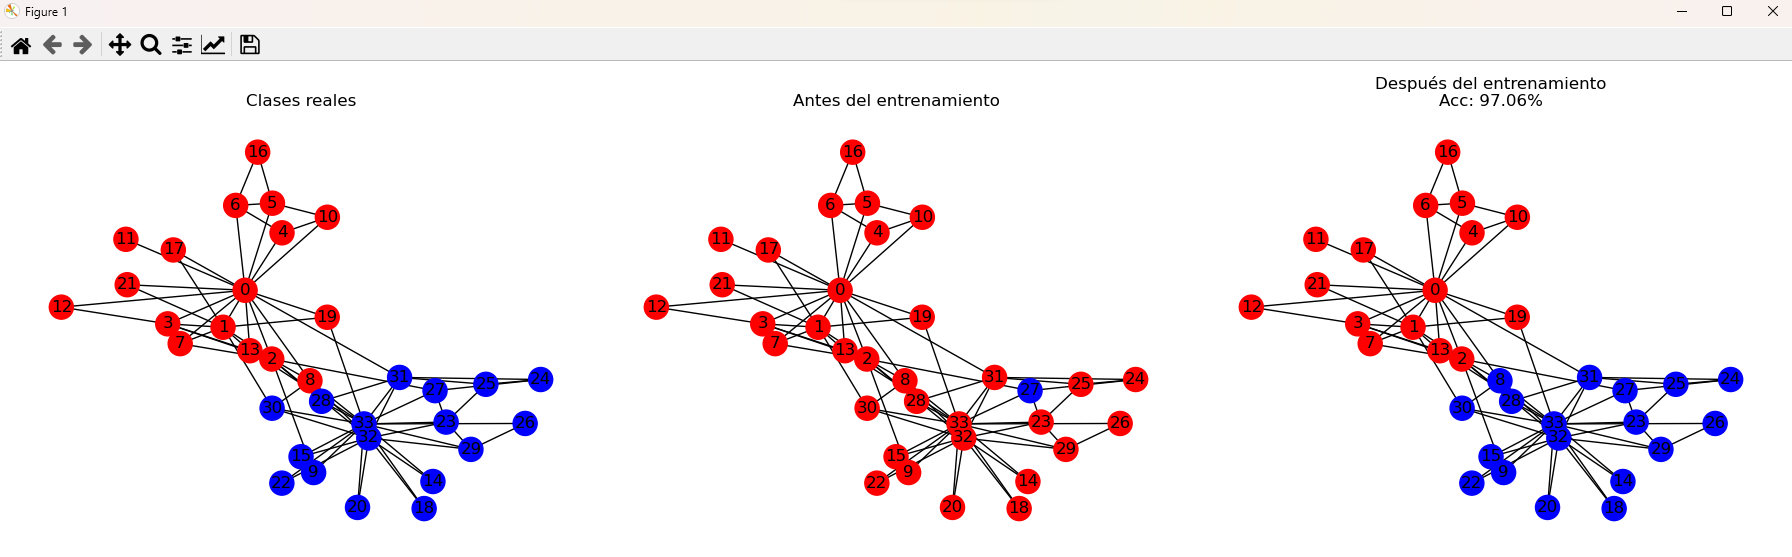
\includegraphics[width=0.9\linewidth]{Images/comparacionGCN.png}
    \caption{Comparación entre el grafo real y las predicciones del modelo GCN}
    \label{fig:comparacionGCN}
\end{figure}

\begin{figure}[H]
    \centering
    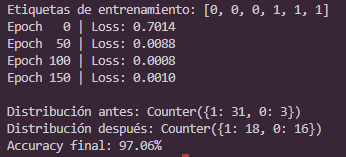
\includegraphics[width=0.7\linewidth]{Images/lossesGCN.png}
    \caption{Evolución de la pérdida durante el entrenamiento del modelo y accuracy final del modelo}
    \label{fig:lossesGCN}
\end{figure}

\newpage


\section{Conclusión}

A lo largo de esta investigación se abordaron los fundamentos y aplicaciones de las Redes Neuronales de Grafos (GNNs), modelos que se han vuelto cada vez más relevantes debido a su capacidad para manejar datos estructurados, es decir, aquellos donde las relaciones entre elementos tienen un papel importante. Desde el inicio, se planteó explorar estos modelos por su potencial en contextos como redes sociales, sistemas de recomendación o grafos de citaciones académicas y entre otras muchas funcionalidades que se tienen.

Primero, se revisaron conceptos básicos como la definición de grafos, su representación mediante matrices y algunas métricas clave. Esto sirvió como base para comprender cómo se estructura la información en forma de red y cómo esta estructura puede ser utilizada en modelos de aprendizaje automático. Luego, se profundizó en los fundamentos de las redes neuronales tradicionales y en las limitaciones que presentan al trabajar con este tipo de datos, lo que permitió entender por qué surgieron las GNNs como una alternativa más adecuada.

Después, se analizaron algunos de los principales modelos dentro del campo de las GNNs, como las GCN (Redes Convolucionales sobre Grafos), las GAT (Redes de Atención en Grafos) y GraphSAGE. Cada uno con su enfoque particular para actualizar las representaciones de los nodos a partir de sus vecinos, demostrando otros tipos de usos de grafos para entreno.

Además, se incluyó un ejemplo práctico utilizando GCN para clasificación de nodos, lo cual permite aterrizar en los conceptos teóricos en un caso concreto. Este ejemplo mostró cómo una red neuronal puede aprender representaciones útiles al combinar información local (de cada nodo) y global (de sus conexiones), lo cual sería difícil de lograr con modelos tradicionales.

En conclusión, las GNNs representan una evolución significativa en el campo del aprendizaje automático, ya que permiten trabajar con estructuras complejas de datos de forma efectiva. Más allá de lo técnico, el estudio también deja claro que este tipo de modelos abre puertas a nuevas soluciones en áreas como la inteligencia artificial aplicada, el análisis de redes, la biología computacional, la ciencia de datos y más. A medida que estas técnicas sigan desarrollándose y mejorando su eficiencia, su impacto en la investigación y la industria continuará creciendo.




\newpage
\section{Referencias}
\nocite{*}
\printbibliography
\newpage 
\section{Anexos}
\vspace{10pt}
\subsection{Anexo A: Glosario de Términos y Conceptos Adicionales}
\subsubsection{Ejemplo de Cálculo de Propagación hacia Adelante}
Dado un vector de entrada \(x = [0.5, -0.3]\), pesos \(W\) y sesgo \(b\):

\[
W = \begin{bmatrix}
0.2 & -0.4 \\
0.7 & 0.1 
\end{bmatrix}, \quad
b = \begin{bmatrix}
0.1 \\
-0.2
\end{bmatrix}
\]

La salida \(y\) se calcula como:
\[
y = \text{ReLU}(Wx + b)
\]

\[
Wx = \begin{bmatrix}
0.2 & -0.4 \\
0.7 & 0.1 
\end{bmatrix}
\begin{bmatrix}
0.5 \\
-0.3
\end{bmatrix}
= \begin{bmatrix}
(0.2)(0.5) + (-0.4)(-0.3) \\
(0.7)(0.5) + (0.1)(-0.3)
\end{bmatrix}
= \begin{bmatrix}
0.1 + 0.12 \\
0.35 - 0.03
\end{bmatrix}
= \begin{bmatrix}
0.22 \\
0.32
\end{bmatrix}
\]

\[
y = \text{ReLU}\left(
\begin{bmatrix}
0.22 \\
0.32
\end{bmatrix} + 
\begin{bmatrix}
0.1 \\
-0.2
\end{bmatrix}
\right)
= \text{ReLU}
\begin{bmatrix}
0.32 \\
0.12
\end{bmatrix}
= \begin{bmatrix}
0.32 \\
0.12
\end{bmatrix}
\]

---

\subsubsection{Glosario de Términos}
\begin{description}
    \item[\textbf{Algoritmo de Optimización}] Método matemático utilizado para minimizar o maximizar una función objetivo, comúnmente la función de pérdida en machine learning.

    \item[\textbf{Batch}] Subconjunto de datos de entrenamiento que se procesa simultáneamente durante una iteración del algoritmo de entrenamiento.
    
    \item[\textbf{Cross-validation (Validación Cruzada)}] Técnica estadística para evaluar la capacidad de generalización de un modelo dividiendo los datos en múltiples particiones.
    
    \item[\textbf{Dropout}] Técnica de regularización que consiste en desactivar aleatoriamente algunas neuronas durante el entrenamiento para prevenir el sobreajuste.
    
    \item[\textbf{Epoch}] Una pasada completa a través de todo el conjunto de datos de entrenamiento.
    
    \item[\textbf{Feature Engineering}] Proceso de selección, modificación o creación de variables (features) a partir de datos en bruto para mejorar el rendimiento del modelo.
    
    \item[\textbf{Gradient Descent}] Algoritmo de optimización iterativo usado para encontrar el mínimo de una función calculando sus gradientes.
    
    \item[\textbf{Hiperparámetros}] Parámetros de configuración del modelo que se establecen antes del entrenamiento y no se aprenden automáticamente.
    
    \item[\textbf{Learning Rate (Tasa de Aprendizaje)}] Hiperparámetro que controla qué tan grande es el paso que da el algoritmo en cada iteración hacia el mínimo de la función de pérdida.
    
    \item[\textbf{Overfitting (Sobreajuste)}] Fenómeno donde el modelo aprende demasiado bien los datos de entrenamiento pero falla al generalizar a datos nuevos.
    
    \item[\textbf{Underfitting (Subajuste)}] Situación donde el modelo es demasiado simple para capturar la estructura subyacente de los datos.
\end{description}
\subsubsection{Funciones de Activación Adicionales}

Además de las funciones mencionadas en el documento principal, existen otras funciones de activación relevantes:

\begin{itemize}
    \item \textbf{Leaky ReLU}: Variante de ReLU que permite un pequeño gradiente cuando la entrada es negativa: $f(x) = \max(0.01x, x)$
    
    \item \textbf{ELU (Exponential Linear Unit)}: $f(x) = \begin{cases} x & \text{si } x > 0 \\ \alpha(e^x - 1) & \text{si } x \leq 0 \end{cases}$
    
    \item \textbf{Swish}: Función autodescubierta por Google: $f(x) = x \cdot \sigma(x)$, donde $\sigma$ es la función sigmoide.
    
    \item \textbf{Softmax}: Utilizada en la capa de salida para problemas de clasificación multiclase: $f(x_i) = \frac{e^{x_i}}{\sum_{j=1}^{K} e^{x_j}}$
\end{itemize}

\subsection{Anexo B. Conceptos complementarios sobre GNNs}

\subsubsection{Fórmula general de una capa GNN}
Una operación de propagación típica en una GNN sigue el siguiente esquema general:

\[
h_i^{(k)} = \sigma \left( \sum_{j \in \mathcal{N}(i)} f\left(h_i^{(k-1)}, h_j^{(k-1)}, e_{ij}\right) \right)
\]

Donde:
\begin{itemize}
    \item $h_i^{(k)}$: representación del nodo $i$ en la capa $k$
    \item $\mathcal{N}(i)$: conjunto de vecinos del nodo $i$
    \item $e_{ij}$: atributo de la arista (si aplica)
    \item $f(\cdot)$: función de agregación o combinación (suma, media, atención, etc.)
    \item $\sigma(\cdot)$: función de activación no lineal (ReLU, tanh, etc.)
\end{itemize}

\subsubsection{Ejemplo numérico de propagación en GCN}
Suponga un grafo de 3 nodos con la siguiente matriz de adyacencia con self-loops:

\[
\tilde{A} = 
\begin{pmatrix}
1 & 1 & 0 \\
1 & 1 & 1 \\
0 & 1 & 1
\end{pmatrix}, \quad
X = 
\begin{pmatrix}
1 & 0 \\
0 & 1 \\
1 & 1
\end{pmatrix}
\]

Con una matriz de pesos $W = 
\begin{pmatrix}
1 & -1 \\
1 & 1
\end{pmatrix}$ y función de activación $\sigma = \text{ReLU}$, el primer paso de propagación sería:

\[
H^{(1)} = \sigma \left( \tilde{A} \cdot X \cdot W \right)
\]

\[
X \cdot W = 
\begin{pmatrix}
1 & -1 \\
1 & 1 \\
2 & 0
\end{pmatrix}, \quad
H^{(1)} = \sigma \left(
\begin{pmatrix}
1 & 1 & 0 \\
1 & 1 & 1 \\
0 & 1 & 1
\end{pmatrix}
\cdot 
\begin{pmatrix}
1 & -1 \\
1 & 1 \\
2 & 0
\end{pmatrix}
\right)
\]

\[
H^{(1)} = \sigma \left(
\begin{pmatrix}
2 & 0 \\
4 & 0 \\
3 & 1
\end{pmatrix}
\right)
=
\begin{pmatrix}
2 & 0 \\
4 & 0 \\
3 & 1
\end{pmatrix}
\]

\subsection{Anexo C. Aspectos Complementarios sobre el Caso de Estudio GCN}

\vspace{10pt}

\subsubsection{Limitaciones Técnicas y Soluciones}

Las GCNs tradicionales presentan algunas limitaciones que han motivado el desarrollo de variantes:

\begin{itemize}
    \item \textbf{Sobreajuste en grafos pequeños:} cuando los datos son escasos, una GCN puede memorizar etiquetas de nodos específicos.
    \item \textbf{Sobre-suavizado (\textit{over-smoothing}):} con muchas capas, las representaciones de los nodos pueden volverse indistinguibles, perdiendo la capacidad de diferenciación.
    \item \textbf{Incapacidad para nodos nuevos:} los modelos transductivos como el original de Kipf y Welling no generalizan automáticamente a nuevos nodos que no estuvieron presentes durante el entrenamiento.
\end{itemize}

\textbf{Soluciones:}
\begin{itemize}
    \item Regularización y técnicas de dropout ayudan a mitigar el sobreajuste.
    \item Usar redes poco profundas (2-3 capas) reduce el sobre-suavizado.
    \item Modelos inductivos como GraphSAGE permiten la generalización a nuevos nodos.
\end{itemize}

\subsubsection{Entornos y Herramientas de Implementación}

Las GCN pueden implementarse con diversas bibliotecas modernas de deep learning:

\begin{itemize}
    \item \textbf{PyTorch Geometric (PyG):} framework sobre PyTorch, ampliamente usado para construir modelos GNN.
    \item \textbf{Deep Graph Library (DGL):} biblioteca flexible que permite trabajar con grafos en PyTorch o TensorFlow.
    \item \textbf{Spektral:} orientado a TensorFlow/Keras, adecuado para prototipos rápidos.
\end{itemize}

Además, conjuntos de datos clásicos como Cora, Citeseer y Pubmed son útiles para realizar experimentos reproducibles. Estos grafos tienen nodos con características textuales y etiquetas de clase.

\subsubsection{Aplicaciones Avanzadas y Futuras Direcciones}

Las GCNs han superado el ámbito de redes sociales y se aplican en:

\begin{itemize}
    \item \textbf{Biología:} predicción de interacciones proteína-proteína, estructuras de moléculas y propiedades químicas.
    \item \textbf{Procesamiento de lenguaje natural:} modelado de dependencias gramaticales o relaciones semánticas entre entidades en textos.
    \item \textbf{Visión por computador:} análisis de escenas, relaciones espaciales entre objetos y reconstrucción 3D.
\end{itemize}

\textbf{Tendencias actuales:} atención gráfica (GATs), GNNs dinámicas para grafos cambiantes en el tiempo, y el uso de GNNs en sistemas multi-agente o simulaciones físicas.

\vspace{10pt}
\noindent En conclusión, las GCN representan una extensión del aprendizaje profundo que permite operar sobre datos no euclidianos, capturando relaciones y patrones complejos que no son accesibles para modelos tradicionales. Su evolución continúa integrando conceptos de atención, memoria y adaptación a grafos dinámicos o heterogéneos.


\end{document}

